\documentclass{article}

\usepackage{arxiv}

\usepackage[utf8]{inputenc} % allow utf-8 input
\usepackage[T1]{fontenc}    % use 8-bit T1 fonts
\usepackage[hidelinks]{hyperref}       % hyperlinks
\usepackage{url}            % simple URL typesetting
\usepackage{booktabs}       % professional-quality tables
\usepackage{amsmath,amssymb,amsthm}
\usepackage{amsfonts}       % blackboard math symbols
\usepackage{nicefrac}       % compact symbols for 1/2, etc.
\usepackage{microtype}      % microtypography
\usepackage{mathrsfs}
\usepackage{graphicx}
\usepackage{doi}
\usepackage{acronym}
\usepackage{listings}
\usepackage{tikz}
\usepackage[backend=biber,style=ieee]{biblatex}

\addbibresource{references.bib}

\usetikzlibrary{trees}

\newacro{abm}[ABM]{Agent-Based Model}
\newacro{cabm}[CABM]{Cellular Agent-Based Model}
\newacro{ca}[CA]{Cellular Automaton}
\newacroplural{ca}[CA]{Cellular Automata}

\title{Rust for Scientific Computing}

%\date{September 9, 1985}	% Here you can change the date presented in the paper title
%\date{} 					% Or removing it

\author{
    \href{https://orcid.org/0009-0001-0613-7978}{
        \includegraphics[scale=0.06]{orcid.pdf}
        \hspace{1mm}Jonas Pleyer
    }
    \thanks{
        \href{https://jonas.pleyer.org}{jonas.pleyer.org},
        \href{https://cellular-raza.com}{cellular-raza.com}
    }\\
	Freiburg Center for Data-Analysis and Modeling\\
	University of Freiburg\\
	\texttt{jonas.pleyer@fdm.uni-freiburg.de} \\
	%% examples of more authors
	\And
	\href{https://orcid.org/0000-0002-6371-4495}{
        \includegraphics[scale=0.06]{orcid.pdf}
        \hspace{1mm}Christian Fleck
    }\\
	Freiburg Center for Data-Analysis and Modeling\\
	University of Freiburg
}

% Uncomment to remove the date
%\date{}

% Uncomment to override  the `A preprint' in the header
\renewcommand{\headeright}{Preprint}
%\renewcommand{\undertitle}{Technical Report}
\renewcommand{\shorttitle}{Rust for High-Performance Computing}

\usepackage{enumitem}
\setlist{nolistsep}

%%% Add PDF metadata to help others organize their library
%%% Once the PDF is generated, you can check the metadata with
%%% $ pdfinfo template.pdf
\hypersetup{
pdftitle={Rust for High-Performance Computing},
pdfsubject={q-bio.NC, q-bio.QM},
pdfauthor={Jonas Pleyer, Christian Fleck},
pdfkeywords={},
}

% Change numbering of equations
% \numberwithin{equation}{section}

% MAKE TITLES IN THEOREMS BOLD
\makeatletter
\def\th@plain{%
  \thm@notefont{}% same as heading font
  \itshape % body font
}
\def\th@definition{%
  \thm@notefont{}% same as heading font
  \normalfont % body font
}
\makeatother

\begin{document}
\maketitle

%###################################################################################################
\begin{abstract}
\end{abstract}

\pagebreak
\tableofcontents
\pagebreak

% keywords can be removed
\keywords{Rust \and HPC \and High-Performance Computing \and Programming}

%###################################################################################################
\section{Introduction}
\label{section:introduction}

\begin{figure}
    \centering
    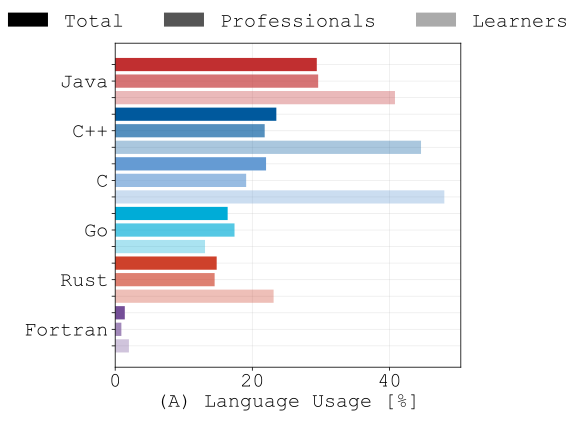
\includegraphics[width=0.5\textwidth]{figures/stackoverflow-popular-languages.pdf}%
    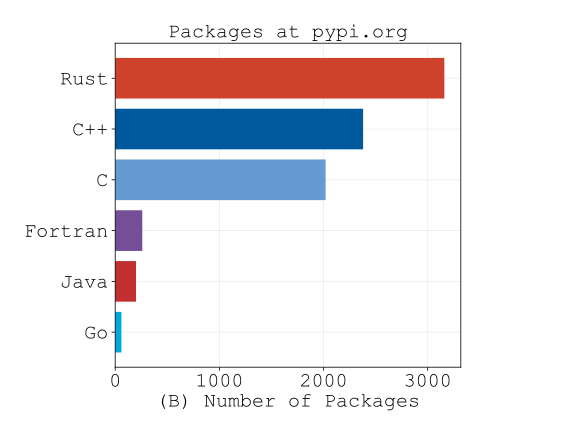
\includegraphics[width=0.5\textwidth]{figures/pypi-org-used-languages.pdf}
    \caption{TODO}
\end{figure}

%###################################################################################################
\section{Ecosystem and Libraries}

\begin{enumerate}
    \item Linear Algebra \& Arrays (nalgebra, ndarray, ...)
    \item Statistics \& Data Analysis (statrs, ndarray-stats, smartcore, ...)
    \item Symbolic \& other Math (num, rug, speciyl, symcc)
    \item ODE solvers~\cite{Renevey2024}, Diffsol
    \item PDE solvers
    \item Fluid Dynamics: Salva (2D \& 3D)~\cite{Crozet2024}
    \item Physics Engine: Rapier (2D \& 3D)~\cite{Crozet2025}
    \item Meshing (honeycomb)
    \item Plotting (plotters, plotlib, gnuplot bindings, vtk-rs)
    \item Utilities (rayon, lapack)
    \item GPU (rust-cuda, wgpu)
    \item Datastructures
    \item Optimization
\end{enumerate}

\subsection{Foundational Components}
\subsubsection{Linear Algebra \& Arrays}
(nalgebra, ndarray) (dense, sparse matrices, solvers)

\subsubsection{Numerical Methods}
(floating point arithmetic, etc.)

\subsubsection{Statistics \& Probability}
(statsrs, ndarray-stats, smartcore)

\subsubsection{Symbolic \& Algebraic Computing}
(num, rug, speciyl, symcc, enzyme)

\subsubsection{Datastructures}
(graphs, etc.)

\subsection{Computational Methods}
\subsubsection{Optimization}
\subsubsection{Differential Equations}
(ODEs, PDEs)

\subsubsection{Physics Engines}
(Fluid Dynamics, Manybody)

\subsubsection{Numerical Integration \& Differentiation}
(quadrature, monte-carlo, symbolic diff, enzyme)

\subsubsection{(Probabilistic Algorithms)}

\subsection{High-Performance \& Scalable Computing}
\subsubsection{Parallel Computing}
(rayon)

\subsubsection{GPU \& Accelerators}
(rust-cuda, wgpu~\cite{Fitzgerald2025})

\subsubsection{Sparse \& Structured Computations}
(large databases)

\subsubsection{Debugging}
(Rust Errors as values, tracing, logging) ecosystem

\subsubsection{Storage}
(serde, json, xml, ron, ...)

\subsection{Visualization}
\subsubsection{Plotting (2D)}
\subsubsection{3D Rendering}
\subsubsection{Interactive}
(dioxus)

%###################################################################################################
\section{Applications}
\label{section:applications}

\subsection{Physics \& Engineering}
\subsection{Biology \& Chemistry}
\cite{Pleyer2024}, Computational Oncology~\cite{Köster2025}, Proteomics~\cite{Anechitoaie2024}
\subsection{Climate \& Earth Sciences}
\subsection{Economics \& Finance}
\subsection{Social Sciences}

%###################################################################################################
\section{Discussion}
\label{section:discussion}

%###################################################################################################
\section{Conclusion}
\label{section:conclusion}

\printbibliography

\end{document}
